\documentclass[tikz]{standalone}
\usepackage{pgfplots}
\pgfplotsset{compat=1.15}
\usepackage{mathrsfs}
\usetikzlibrary{arrows,calc}
\usepackage{tkz-euclide}

\pagestyle{empty}

\definecolor{AngleClr}{rgb}{0,0.39215686274509803,0}
\definecolor{ShapeClr}{rgb}{0.6,0.2,0}
\definecolor{ParacircleClr}{RGB}{217,185,7}

\begin{document}

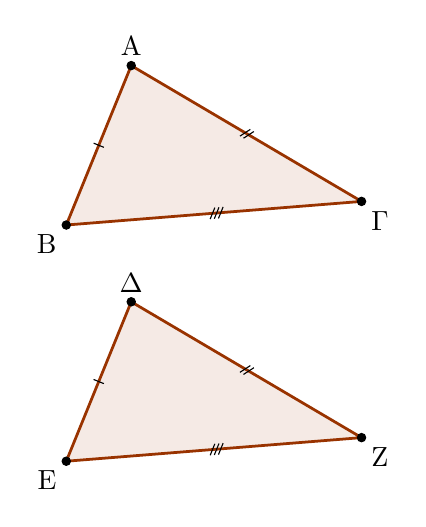
\begin{tikzpicture}[scale=.75]
\tkzSetUpLine[line width=1pt,color=black]
\tkzSetUpPoint[fill=black]

\tkzDefPoints{0/0/B,1.1/2.7/A,5/0.4/C}
\tkzDefPoints{0/-4/E,1.1/-1.3/D,5/-3.6/Z}

\tkzFillPolygon[fill=ShapeClr,fill opacity=0.1](A,B,C)
\tkzFillPolygon[fill=ShapeClr,fill opacity=0.1](D,E,Z)

\tkzDrawPolygon[color=ShapeClr](A,B,C)
\tkzDrawPolygon[color=ShapeClr](D,E,Z)

\tkzDrawPoints[size=3](A,B,C,D,E,Z)

\tkzLabelPoint[above](A){$\rm A$}
\tkzLabelPoint[below left](B){$\rm B$}
\tkzLabelPoint[below right](C){$\rm \Gamma$}

\tkzLabelPoint[above](D){$\rm \Delta$}
\tkzLabelPoint[below left](E){$\rm E$}
\tkzLabelPoint[below right](Z){$\rm Z$}

\tkzMarkSegments[mark=|,size=2](A,B E,D)
\tkzMarkSegments[mark=s||,size=2](A,C D,Z)
\tkzMarkSegments[mark=s|||,size=2](B,C E,Z)


\end{tikzpicture}
\end{document}
